\scanpage{416}

Composition with the canonical projection to
$T_\rho\times N'_\sigma$ gives a \uline{monomorphism}

\margin{for we shall have
\diagram{\begin{tikzcd}[ampersand replacement=\&]
T_0 \arrow[r,"{\substack{\det\\\sim}}"] \& \mathbb G_m
\end{tikzcd}}}

\[
(24)\qquad
\diagram{\begin{tikzcd}[ampersand replacement=\&,column sep=large]
\mathcal T_{\rho,\sigma} \arrow[r,hook] \arrow[d,phantom,"{\rotatebox{90}{$\simeq$}}" description]
 \& T_\rho\times N'_\sigma \\
\left\{(\underline a,\underline b)\mid
 (\det\underline a/\det\underline b)^2=1\right\}
 \& \inserted{\left.\begin{gathered}
\text{i.e. }\det\underline a=\varepsilon'\det\underline b\\
\text{with }\varepsilon'^2=1
\end{gathered}\right\}}
\end{tikzcd}}
\]

and we shall therefore have
\[
(25)\qquad
\left\{\begin{aligned}
\chi(\underline a,\underline b)&=\det\underline b\\
\varepsilon_2(\underline a,\underline b)&=\varepsilon_\sigma(\underline b)\\
\varepsilon_3(\underline a,\underline b)&=\det(\underline a)/\det(\underline b)
 =\det\underline b/\det\underline a
\end{aligned}\right.
\]

We define
\[
(26)\qquad
\diagram{\begin{tikzcd}[ampersand replacement=\&,column sep=small]
\mathcal T_{\rho,\sigma}^{\circ} \arrow[d,phantom,"{\rotatebox{90}{$\simeq$}}" description]
 \& {}=\operatorname{Ker}\mathcal T_{\rho,\sigma}
 \arrow[r,"{(\varepsilon_2,\varepsilon_3)}"]
 \& \mu_2\times\mu_2 \\
\inserted{T_\rho\times_{\mathbb G_m}T_\sigma} \&\&
\end{tikzcd}}
\]
so we have
\[
(27)\qquad
\diagram{\begin{tikzcd}[ampersand replacement=\&]
1 \arrow[r] \& \mathcal T_{\rho,\sigma}^{\circ} \arrow[r]
 \& \mathcal T_{\rho,\sigma} \arrow[r] \& \mu_2\times\mu_2 \arrow[r] \& 1
\end{tikzcd}}
\]
and a canonical exact sequence
\[
(28)\qquad
\diagram{\begin{tikzcd}[ampersand replacement=\&]
1 \arrow[r] \&
\overbrace{ST_\rho\times ST_\sigma}^{\inserted{\mathcal T_{\rho,\sigma}^{\circ+}}}
\arrow[r] \& \mathcal T_{\rho,\sigma}^{\circ} \arrow[r,"{\chi}"]
 \& \mathbb G_m \arrow[r] \& 1,
\end{tikzcd}}
\]
where we define
\[
(29)\qquad
\left\{\begin{aligned}
ST_\rho&=\{g\in\Gamma T_\rho\mid\det g=1\}\\
ST_\sigma&=\{g\in\Gamma T_\sigma\mid\det g=1\}
\end{aligned}\right.\quad.
\]

\margin{\figure{\begin{tikzpicture}[x=.65cm,y=.65cm]
\draw[->] (0,4.5) .. controls (1.1,4.55) and (1.1,3.7) .. (1.1,3.25)
 -- (1.2,.8) .. controls (1.2,.45) and (1.55,.55) .. (2.4,.65);
\draw (0,0) .. controls (1.0,-.05) and (1.05,.1) .. (1.15,.45)
 .. controls (1.25,.75) and (1.55,.65) .. (2.4,.65);
\end{tikzpicture}}}
\inserted{The operation of $\mathcal T_{\rho,\sigma}\simeq
\mathcal M_{\rho,\sigma}(0)$ on $L_0$ is given by
\[
(30)\qquad g(\varepsilon_0(\lambda))=\varepsilon_0(\mu\lambda),
\quad\text{where }\mu=\chi(g)
\]}

We let $\mathcal M_{\rho,\sigma}(0)
(\simeq\mathcal T_{\rho,\sigma})$ operate on $SG$, by
\[
(31)\qquad
\diagram{\begin{tikzcd}[ampersand replacement=\&,column sep=large]
\mathcal M_{\rho,\sigma}(0)
 \arrow[r,"{\text{projection}}"]
 \& T_0 \arrow[r,"{\substack{\text{canonical}\\(\text{monomorphism})}}"]
 \& PG \arrow[r,"{\sim}"]
 \& \underline{\operatorname{Aut}}_{\mathrm{gr}}(SG) \\
T_0\times T_\rho\times N'_\sigma \arrow[u,phantom,"{\cap}" description]
 \& G \arrow[u,phantom,"{\cap}" description]
 \& G/\mathbb G_m\simeq\underline{\operatorname{Aut}}(G)
 \arrow[u,phantom,"{\rotatebox{90}{$\simeq$}}" description] \&
\end{tikzcd}}
\]

\par\noindent 415

\scanpage{417}
\mspage{510}

and we define
\[
(32)\qquad \mathcal M_{\rho,\sigma}\simeq
 \mathcal M_{\rho,\sigma}(0)\mathbin{.}SG
\]
\hfill $\frac12$ direct product

We thus have a canonical homomorphism
\[
(33)\qquad
\diagram{\begin{tikzcd}[ampersand replacement=\&]
SG \arrow[r,hook,"{j}"] \& \mathcal M_{\rho,\sigma}
\end{tikzcd}}
\]
whose image is denoted $\widetilde{\mathcal G}_{\rho,\sigma}^{+}$, so
\[
(34)\qquad
\diagram{\begin{tikzcd}[ampersand replacement=\&]
1 \arrow[r] \& \widetilde{\mathcal G}_{\rho,\sigma}^{+} \arrow[r]
 \& \mathcal M_{\rho,\sigma} \arrow[r] \& \mathcal T_{\rho,\sigma} \arrow[r] \& 1
\end{tikzcd}}
\]
\[
(35)\qquad
\diagram{\begin{tikzcd}[ampersand replacement=\&,column sep=0.3em,row sep=1.3em]
\mathcal M_{\rho,\sigma}\simeq \& \mathcal M_{\rho,\sigma}(0)
 \arrow[d,phantom,"{\rotatebox{90}{$\simeq$}}" description]
 \& {}\mathbin{.}\widetilde{\mathcal G}_{\rho,\sigma}^{+} \\
 \& \mathcal T_{\rho,\sigma} \&
\end{tikzcd}}
\]
\hfill $\frac12$ direct product.

\uline{N.B.} We use the notation $\mathcal T_{\rho,\sigma}$ for the
quotient group
\[
(36)\qquad \mathcal T_{\rho,\sigma}\simeq
\mathcal M_{\rho,\sigma}/\widetilde{\mathcal G}_{\rho,\sigma}^{+},
\]
the notation $\mathcal M_{\rho,\sigma}[0)$ for the subgroup
of $\mathcal M_{\rho,\sigma}$.

We define a canonical embedding
\[
(37)\qquad
\diagram{\begin{tikzcd}[ampersand replacement=\&]
\mathcal M_{\rho,\sigma}[0] \arrow[r,hook,"{i}"] \& \mathcal M_{\rho,\sigma}
\end{tikzcd}}
\]
which extends the inclusions \unsure{of the subgroups|of the subgroup}
$\mathcal M_{\rho,\sigma}(0)$ common to $\mathcal M_{\rho,\sigma}[0]$
and to $\mathcal M_{\rho,\sigma}$,
and which on $L_0$ is given by
\[
(38)\qquad i(\lambda)=j(\lambda)\qquad (\text{cf. }(33))
\]
(which is indeed compatible with the operations of
$\deleted{\unsure{\mathcal T|\mathcal M}}\mathcal M_{\rho,\sigma}(0)$
on $L_0$ on the one hand, on $SG\simeq\widetilde{\mathcal G}_{\rho,\sigma}^{+}$
on the other).

\par\noindent 416

\scanpage{418}

Another way of saying it is to observe that
$\mathcal M_{\rho,\sigma}(0)$ operating on
$SG\simeq\widetilde{\mathcal G}_{\rho,\sigma}^{+}$
normalizes the subgroup $j(L_0)$ -- which we
henceforth identify with $L_0$), so that we
shall have a subgroup
\[
\mathcal M_{\rho,\sigma}(0)\mathbin{.}L_0\subset\mathcal M_{\rho,\sigma}
\]
which \unsure{is|will be} canonically isomorphic to $\mathcal M_{\rho,\sigma}[0]$
defined above, thanks to the expression $(\unsure{19|49})$ of
the latter as a $\frac12$-direct product.

\deleted{\uline{Proposition}}
\inserted{\uline{Remark.}} We have
\[
\deleted{(\unsure{39})}\qquad
\mathcal M_{\rho,\sigma}[0]\subset
\underline{\operatorname{Norm}}_{\mathcal M_{\rho,\sigma}}(L_0)
\]

By construction, \deleted{\unsure{we have} $\subset$, \unsure{for} $\unsure{\supset}$}
the inclusion in the reverse direction would amount to saying that $L_0$
is its own normalizer in $SG\simeq\widetilde{\mathcal G}_{\rho,\sigma}^{+}$,
which of course is not true at all
-- \unsure{even} though the analogous fact is true
in the profinite group
$\widetilde{\mathcal G}_{0,3}^{\widehat{+}}$,
for the subgroup generated by $\varepsilon_0$,
or in $\Pi_{0,\widehat{3}}$ for
the one generated by $l_0$ (\unsure{subject to} verification !
besides which I still haven't done).

\par\noindent 417

\scanpage{419}
\mspage{511}

\margin{$\mathcal M_{\rho,\sigma}^{\circ},\mathcal M_{\rho,\sigma}^{+},
\mathcal M_{\rho,\sigma}^{+\circ},\mathcal T_{\rho,\sigma}^{\circ},
\mathcal T_{\rho,\sigma}^{+},\mathcal T_{\rho,\sigma}^{\circ+}\ldots$
some central subgroups and computations of integral \unsure{points}\ldots}

\figure{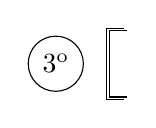
\begin{tikzpicture}[baseline=(n.base)]
\node[draw,circle,inner sep=3pt] (n) at (0,0) {$3^{\mathrm o}$};
\draw[line width=.6pt] (.90,.42)--(.68,.42)--(.68,-.42)--(.90,-.42);
\draw[line width=.45pt] (.86,.45)--(.64,.45)--(.64,-.45)--(.86,-.45);
\end{tikzpicture}}
We denote by $\mathcal M_{\rho,\sigma}^{\circ}$,
$\mathcal M_{\rho,\sigma}[0]^{\circ}$,
$\deleted{\unsure{\mathcal M}}\mathcal M_{\rho,\sigma}[0)^{\circ}$
identity components, we shall have for example
\[
(39)\qquad
\diagram{\begin{tikzcd}[ampersand replacement=\&,column sep=small]
1 \arrow[r] \& \mathcal M_{\rho,\sigma}^{\circ}
 \arrow[r] \arrow[d,phantom,"{\rotatebox{90}{$\simeq$}}" description]
 \& \mathcal M_{\rho,\sigma} \arrow[r] \& \mu_2\times\mu_2 \arrow[r] \& 1\\
 \& \mathcal M_{\rho,\sigma}^{\circ}(0)\mathbin{.}\widetilde{\mathcal G}_{\rho,\sigma}^{+}
 \&\&\&
\end{tikzcd}}
\]
\hspace*{4em} $\frac12$ direct product
\[
(40)\qquad
\diagram{\begin{tikzcd}[ampersand replacement=\&]
\mathcal M_{\rho,\sigma}(0)^{\circ} \arrow[r,"{\sim}"]
 \& \mathcal T_{\rho,\sigma}^{\circ}\simeq T_\rho\times_{\mathbb G_m}T_\sigma
\end{tikzcd}}
\]
\[
(41)\qquad
\begin{gathered}
\mathcal M_{\rho,\sigma}^{\circ}\text{ is the inverse image of }
\mathcal T_{\rho,\sigma}^{\circ}\\
\text{under }\diagram{\begin{tikzcd}[ampersand replacement=\&]
\mathcal M_{\rho,\sigma} \arrow[r,"{\text{canonical}}"] \& \mathcal T_{\rho,\sigma}
\end{tikzcd}},
\end{gathered}
\]

we have a canonical composite homomorphism
\[
(42)\qquad
\diagram{\begin{tikzcd}[ampersand replacement=\&]
\mathcal M_{\rho,\sigma} \arrow[r] \& \mathcal T_{\rho,\sigma}
 \arrow[r,"{\chi}"] \& \mathbb G_m
\end{tikzcd}}
\]
also denoted $\chi$, its kernel is denoted
$\mathcal M_{\rho,\sigma}^{+}$, and we define in the $=$ way
$\mathcal M_{\rho,\sigma}^{\circ+}$, so
\[
(43)\qquad
\diagram{\begin{tikzcd}[ampersand replacement=\&]
1 \arrow[r] \& \mathcal M_{\rho,\sigma}^{+} \arrow[r]
 \arrow[d,phantom,"{\unsure{\cup|\downarrow}}" description]
 \& \mathcal M_{\rho,\sigma} \arrow[r,"{\chi}"]
 \arrow[d,phantom,"{\unsure{\cup|\downarrow}}" description]
 \& \mathbb G_m \arrow[r]
 \arrow[d,phantom,"{\unsure{\cup|\downarrow}}" description] \& 1\\
1 \arrow[r] \& \mathcal M_{\rho,\sigma}^{\circ+} \arrow[r]
 \& \mathcal M_{\rho,\sigma}^{\circ} \arrow[r,"{\chi}"]
 \& \mathbb G_m \arrow[r] \& 1
\end{tikzcd}}
\]
\[
(44)\qquad
\left\{\begin{aligned}
\mathcal M_{\rho,\sigma}^{+}&\simeq
\underbrace{\mathcal M_{\rho,\sigma}^{+}(0)}_{
\substack{\rotatebox{90}{$\simeq$}\\\mathcal T_{\rho,\sigma}^{+}}}
\mathbin{.}\widetilde{\mathcal G}_{\rho,\sigma}^{+}\\[3em]
\mathcal M_{\rho,\sigma}^{\circ+}&\simeq
\underbrace{\mathcal M_{\rho,\sigma}^{\circ+}(0)}_{
\substack{\rotatebox{90}{$\simeq$}\\
\mathcal T_{\rho,\sigma}^{\circ+}\simeq ST_\rho\times ST_\sigma\\
\text{cf. }(28)}}
\mathbin{.}\widetilde{\mathcal G}_{\rho,\sigma}^{+}
\end{aligned}\right.
\]

Thus we have
\[
(45)\qquad
\begin{gathered}
\mathcal M_{\rho,\sigma}^{\circ+}(0)\overset{\mathrm{dfn}}=
\operatorname{Ker}\left(\diagram{\begin{tikzcd}[ampersand replacement=\&]
\mathcal M_{\rho,\sigma}^{\circ}(0)
 \arrow[r,"{{\chi,\varepsilon_2,\varepsilon_3}}"]
 \& \mathbb G_m\times\mu_2\times\mu_2
\end{tikzcd}}\right)\\
\simeq ST_\rho\times ST_\sigma
\end{gathered}
\]
and this subgroup is \uline{central} in
$\mathcal M_{\rho,\sigma}^{\circ}$
(not in $\mathcal M_{\rho,\sigma}$), more precisely

\par\noindent 418

\scanpage{420}

we have
\[
\begin{aligned}
(46)\qquad
\mathcal M_{\rho,\sigma}^{\circ+}
&\overset{\mathrm{dfn}}{=}
\operatorname{Ker}\bigl(\mathcal M_{\rho,\sigma}
\xrightarrow{(\chi,\varepsilon_2,\varepsilon_3)}
\mathbb G_m\times\mu_2\times\mu_2\bigr)
\deleted{\unsure{\simeq}}\\
&\simeq
\underbrace{ST_\rho\times ST_\sigma}_{\subset\mathcal M_{\rho,\sigma}(0)}
\times\widetilde{\mathcal G}_{\rho,\sigma}^{+}
\end{aligned}
\]

\margin{The whole end of the number should come
after (or before) \unsure{the} number $6^\circ$
\unsure{about} the ``\unsure{radicalities}''}

\margin{$\circ$ Careful, this inclusion is not an equality,
cf. below\ldots}

\[
(47)\qquad
\uline{\operatorname{Centr}}(\mathcal M_{\rho,\sigma}^{\circ})
\supset
\underbrace{1\times ST_\rho\times ST_\sigma}_{\substack{\cap\\
\mathcal M_{\rho,\sigma}(0)^\circ}}
\times
\underset{\substack{\cap\\\widetilde{\mathcal G}_{\rho,\sigma}^{+}\simeq SG}}{\mu_2}.
\]

Hence a subgroup
\[
(48)\qquad
\mu_2\times\mu_2\times\mu_2
\subset 1\times
\underbrace{ST_\rho\times ST_\sigma\times\mu_2}_{\substack{\cap\\
\operatorname{Centr}(\mathcal M_{\rho,\sigma}^{\circ})}}
\]
which is in fact contained in the Center of $\mathcal M_{\rho,\sigma}$
as a whole, for
\[
(49)\qquad
\uline{\operatorname{Centr}}(\mathcal M_{\rho,\sigma})
\supset
\underbrace{1\times S'T_\rho\times\mu_2}_{\substack{\cap\\
\mathcal M_{\rho,\sigma}(0)}}
\times
\underset{\substack{\cap\\\widetilde{\mathcal G}_{\rho,\sigma}^{+}\simeq SG}}{\mu_2}
\]
\margin{\unsure{id.}}
with
\[
(50)\qquad
S'T_\rho\overset{\mathrm{dfn}}{=}
\{g\in\Gamma T_\rho\mid(\det g)^2=1\}
\]
so that we have
\diagram{\begin{tikzcd}[ampersand replacement=\&,column sep=large]
\text{(51)}\quad 1 \arrow[r] \& ST_\rho \arrow[r] \&
S'T_\rho \arrow[r,"{\varepsilon_3}"] \& \mu_2 \arrow[r] \& 1
\end{tikzcd}}

We thus have
\[
(52)\qquad
\operatorname{Centr}(\mathcal M_{\rho,\sigma})\cap
\mathcal M_{\rho,\sigma}^{\circ}
\supset
\underset{\substack{\cap\\T_0}}{1}\times
\underset{\substack{\cap\\T_\rho}}{ST_\rho}\times
\underset{\substack{\cap\\T_\sigma}}{\mu_2}\times
\underset{\substack{\cap\\\widetilde{\mathcal G}_{\rho,\sigma}^{+}}}{\mu_2}.
\]
\margin{\unsure{id.}}

The ``modular case'' is the one where
\[
(53)\qquad
\left\{\begin{aligned}
\det\rho&=1\quad\text{i.e.}\quad\det\sigma=1
\quad\text{i.e.}\quad\nu=-1\\
\text{i.e.}\quad\rho&=\begin{pmatrix}0&1\\-1&1\end{pmatrix}
\quad\text{i.e.}\quad\sigma=\begin{pmatrix}0&1\\-1&0\end{pmatrix}
\end{aligned}\right.
\]
(cf. \uline{$\overline{\mathrm{VI}}$} for other
characterizations, such as
$\sigma^2=-1$, or $\rho^2-\rho+1=0$, or
$\widetilde\sigma^2=\widetilde\rho^3=1\ldots$),
this also means that $\rho$ (as an element of $T_\rho$)
is in $ST_\rho$ hence in the \unsure{center} of $\mathcal M_{\rho,\sigma}^{\circ}$,

\par\noindent 419